%%%%%%%%%%%%%%%%%%%%%%%%%%% asme2e.tex %%%%%%%%%%%%%%%%%%%%%%%%%%%%%%%
% Template for producing TSFP-format articles using LaTeX
% Based on the asme2e template (http://iel.ucdavis.edu/code/ASME/)
% Modified: 30 January 2011 for TSFP7 by C. Vanderwel
% Modified: 11 February 2013 for TSFP8 by R. Manceau
% Modified: 05 May 2014 for TSFP9&10 by K. Chauhan (kapil.chauhan@sydney.edu.au)
% Modified: 15 May 2018 for TSFP11 by C. Vanderwel (c.m.vanderwel@soton.ac.uk)
% Modified: 16 December 2024 for TSFP14 by K. V. Wilhelm (wilhelm@fdy.tu-darmstadt.de)
%%%%%%%%%%%%%%%%%%%%%%%%%%%%%%%%%%%%%%%%%%%%%%%%%%%%%%%%%%%%%%%%%%%%%%

%%%%%%%%%%%%%%%%%%%%%%%%%%%%%%%%%%%%%%%%%%%%%%
% To generate a pdf, compile either with pdflatex
% or with latex and
% dvips tsfp_template -Ppdf -t a4 -o
% followed by
% ps2pdf tsfp_template.ps
% (avoid using dvipdf that does not preserve the page layout on some systems)
%%%%%%%%%%%%%%%%%%%%%%%%%%%%%%%%%%%%%%%%%%%%%%

%%% use twocolumn and 10pt options with the tsfp format
\documentclass[twocolumn,10pt]{tsfp}
\usepackage{flushend}
\usepackage{graphicx}
\usepackage[authoryear,round]{natbib}
\usepackage{fancyhdr}
\usepackage{../../preamble_math}
% \usepackage{subcaption}
\usepackage{bm}

 %%%%%%%%%% additional definitions %%%%%%%%%%
\newcommand\dstar{{\delta^*}} % displacement thickness
\newcommand\cc{\text{c.c.}} % complex conjugate


\pagestyle{fancy}
\fancyhf{}
\renewcommand{\headrulewidth}{0pt}
\chead{14th International Symposium on Turbulence and Shear Flow Phenomena (TSFP14) \\ Heidelberg, Germany, July 28--31, 2026}
\cfoot{\thepage}


\title{Transition mechanisms in laminar boundary layers over surface gaps}

%%%% In case you need to slightly adapt the horizontal spacing between authors (for more than 3 authors) uncomment the following command
%%%% and if necessary modify the factor
%\renewcommand{\expauthors}{1.1}

%%% first author
\author{Víctor Ballester Ribó
\affiliation{
    Department of Aeronautics\\
    Imperial College London\\
    London, UK\\
vb824@ic.ac.uk
}	
}

%%% second author
%%% remove the following entry for single author papers
%%% add more entries for additional authors
\author{Jeffrey D. Crouch
      \affiliation{\\
    The Boeing Company\\
    Seattle, USA\\
    jeffrey.d.crouch@boeing.com
}
}


%%% third author
%%% remove the following entry for single author papers
%%% add more entries for additional authors
\author{Yongyun Hwang
		  \affiliation{Department of Aeronautics\\
	Imperial College London\\
	London, UK\\
	y.hwang@imperial.ac.uk
	}
}

%%% fourth author
%%% remove the following entry for single author papers
%%% add more entries for additional authors
\author{Spencer J. Sherwin
		  \affiliation{Department of Aeronautics\\
	Imperial College London\\
	London, UK\\
	s.sherwin@imperial.ac.uk
	}
}


\begin{document}

\maketitle   %Print title matter
\thispagestyle{fancy}

% Set the font to 9pt.
\fontsize{9}{11}\selectfont

%%%%%%%%%%%%%%%%%%%%%%%%%%%%%%%%%%%%%%%%%%%%%%%%%%%%%%%%%%%%%%%%%%%%%%
\section*{ABSTRACT}

This paper presents a combined numerical and stability analysis of transition in laminar boundary layers over surface gaps. High-order spectral/$hp$ simulations are used to map the response to gap width and depth in both the incompressible and compressible regime, while linearised analyses quantify Tollmien--Schlichting (TS) wave amplification within the classical $e^n$ framework. The results show a depth-dependent Hopf onset, followed by periodic and, at larger widths, chaotic two-dimensional dynamics. Predicted $\Delta n$ levels agree closely with available experiments and recover the known shallow- and deep-gap asymptotic trends. Three-dimensional computations further reveal distinct transition routes: for deep gaps, weak low-frequency spanwise modes precede rapid breakdown once the two-dimensional oscillatory mode destabilizes; for shallow gaps, transition continues to be governed by TS-wave downstream of the gap. Compressible flow simulations demonstrate a clear free-stream Mach-number ($\Ma$) influence on the bifurcation boundary, with increasing Mach-number generally reducing the critical width but with non-monotonic behavior for shallow geometries at $\Ma=0.8$. These results provide a unified view of gap-induced transition across two- and three-dimensional, incompressible and compressible conditions.

\section*{INTRODUCTION}
Aircraft aerodynamic surfaces are not perfectly smooth and often contain small geometric discontinuities, commonly referred to as gaps. Although these imperfections are typically small, they can substantially modify boundary-layer development and advance laminar--turbulent transition.

Several studies have examined the effect of surface gaps and cavities on transition. ONERA (\emph{Office National d'Études et de Recherches Aérospatiales}) has conducted extensive experimental, numerical, and theoretical campaigns on this topic; a comprehensive summary is given by~\cite{beguetONERA}. Gap geometry is characterized by $w/\delta^*$ and $d/\delta^*$, where $w$ and $d$ are the gap width and depth, and $\delta^*$ is the boundary-layer displacement thickness at the start of the gap. In~\cite{beguetONERA}, vortex structures inside the gap are classified as functions of $w$ and $d$ for aspect ratios $d/w \in [0.2, 0.7]$. Using the notation $\Delta n = n-n_0$, where $n$ is the gapped-case $n$-factor and $n_0$ corresponds to a smooth flat plate, two main effects are reported: amplification of pre-existing TS waves downstream of the gap, and localized instability generation at the gap itself. Their results were obtained under incompressible conditions.

\cite{zahnRist} investigated deep gaps ($d/w \geq 5$) in compressible boundary layers at $\Ma=0.6$ and reported non-monotonic variations of $\Delta n$ with gap depth, with values between 0 and 0.5. More broadly,~\cite{dynandcontrol} reviewed methods for analyzing and controlling cavity flows in high-Reynolds-number compressible regimes, emphasizing the coupling among shear-layer instabilities, acoustic feedback, and cavity recirculation, all of which are relevant to deep-gap dynamics.

One of the most detailed recent studies is that of~\cite{jeffGaps}, which systematically quantified TS-wave amplification over a broad range of gap widths and depths. For shallow gaps ($d/w < 0.017$), $\Delta n$ depends primarily on depth and is nearly independent of width. For deeper gaps ($d/w > 0.028$), $\Delta n$ is primarily controlled by width. When both $d$ and $w$ are sufficiently large, TS-wave-mediated transition is bypassed and breakdown occurs close to the downstream gap edge. Their results also indicate that shallow-gap behavior resembles that of an isolated backward-facing step.

In this work, we perform a systematic study of surface-gap-induced transition by varying both gap width and depth. We combine direct numerical simulation (DNS) and linear stability analysis in the incompressible regime, and benchmark the results against the experimental trends reported in~\cite{jeffGaps}. We then extend the analysis to three dimensions and to compressible flow in order to examine transition pathways and Mach-number effects on the instability boundaries.

Transition modeling is based on the classical $e^n$ framework, in which linear disturbances (typically TS waves) amplify downstream according to $A(x)=A(x_0)\mathrm{e}^{n(x)}$. Transition is assumed once a critical amplification level is reached. To quantify the gap effect, we use $\Delta n$, defined as the difference between the $n$-factors of the gapped and smooth-wall configurations.

Computationally, the incompressible equations are solved with a spectral/$hp$ element method that combines finite-element geometric flexibility with spectral accuracy. All simulations are carried out in the open-source \texttt{Nektar++} framework (see~\cite{nektar}).

\section*{NUMERICAL FRAMEWORK}
The incompressible Navier--Stokes equations are solved with a spectral/$hp$ element formulation. In nondimensional form, the governing equations are
\begin{equation}
	\begin{aligned}
		\partial_t \mathbf{u} + \mathbf{u} \cdot \grad \mathbf{u} & = -\grad p + \frac{1}{\Rey} \laplacian \mathbf{u}, \\
		\grad \cdot \mathbf{u}                                    & = 0,
	\end{aligned}
\end{equation}
where $\mathbf{u}=(u,v)$ or $\mathbf{u}=(u,v,w)$ is the velocity field for two- or three-dimensional configurations, respectively, $p$ is the pressure, and $\Rey$ is the Reynolds number. The nondimensionalisation uses the free-stream velocity $u_\infty$ and the displacement thickness $\dstar$ at the upstream gap location of the smooth-wall reference flow as characteristic velocity and length scales. With this choice,
\(
\Rey=u_\infty \dstar/\nu,
\)
where $\nu$ is the kinematic viscosity. Throughout the incompressible study, $\Rey=1000$.

For the incompressible simulations, the \texttt{Nektar++} solver is configured with a velocity-correction scheme and continuous Galerkin projection. Time integration is second-order IMEX, with explicit treatment of nonlinear advection and implicit treatment of viscous terms. A polynomial order of $p=5$ and $p=4$ is used for the velocity and pressure fields, respectively. The resulting spatial resolution is sufficient to resolve all relevant flow features, as verified by grid-convergence studies.

The computational domain is rectangular, with a cavity attached to the lower wall to model the surface gap (Figure~\ref{fig:domain}). The dimensions $h=150\dstar$, $\ell_{\text{i}}=100\dstar$, and $\ell_{\text{o}}=1000\dstar$ are selected to ensure a fully developed upstream boundary layer and negligible influence of the downstream boundary on the region of interest. Boundary conditions are a Blasius profile at the inlet, no-slip on solid walls ($\mathbf{u}=\mathbf{0}$), and far-field conditions at the upper boundary ($\mathbf{u}=\mathbf{u}_\infty(x)$).~\cite{dong} outflow boundary condition is applied at the outlet to minimize numerical instabilities when energetic vortices pass through the outflow region.

\begin{figure}[ht]
	\centering
	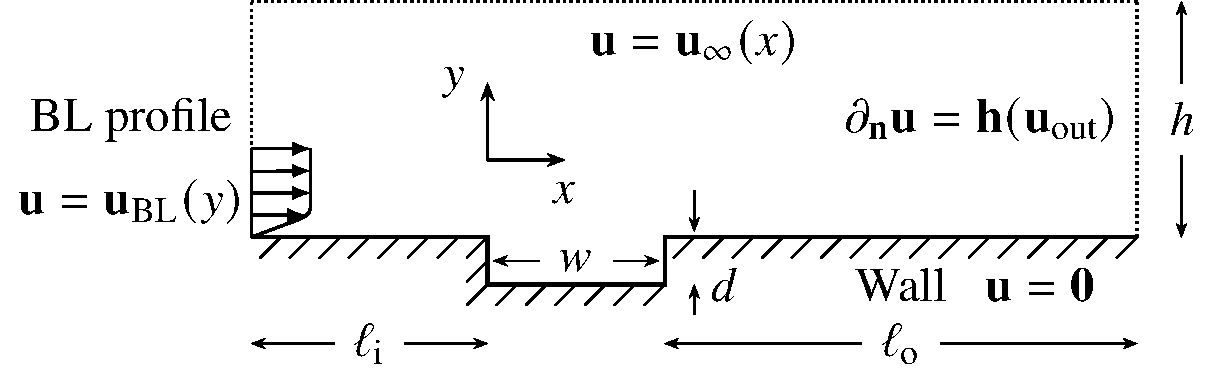
\includegraphics[width=\linewidth]{Images/domainBaseflowExtended.pdf}
	\caption{Computational domain and boundary conditions for two-dimensional nonlinear simulations. Dimensions are anisotropically rescaled for clearer visualization of the gap geometry.}\label{fig:domain}
\end{figure}

\section*{NONLINEAR DYNAMICS AND BIFURCATIONS}

We consider two-dimensional configurations spanning $10\leq w/\dstar \leq 130$ and $0.25 \leq d/\dstar \leq 4$. For each geometry, simulations are initialized from smooth fields, integrated to their limit set, and classified as shown in Figure~\ref{fig:2dstability}.
\begin{figure}[ht]
	\centering
	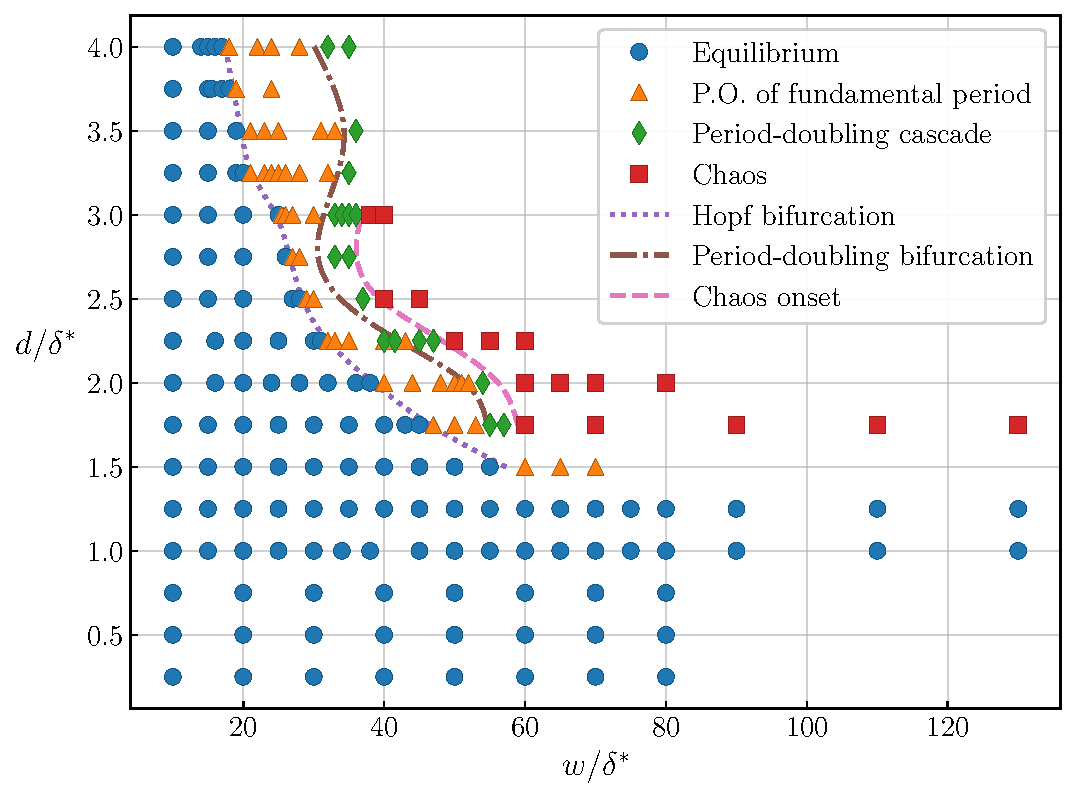
\includegraphics[width=\linewidth]{../../../images/inc2dStabilityCurve.pdf}
	\caption{Limit set classification over the parameter space $10\leq w/\dstar \leq 130$ and $0.25 \leq d/\dstar \leq 4$. Blue circles denote equilibrium states, orange triangles denote limit cycles, and green diamonds denote chaotic attractors.}\label{fig:2dstability}
\end{figure}

As expected, sufficiently small gaps (in either width or depth) yield stable dynamics close to the flat-plate limit ($d\to 0$ or $w\to 0$).

The internal cavity topology varies strongly with geometry. Outside the gap, the boundary layer remains Blasius-like, whereas inside the gap the streamline structure depends on the available cavity volume. Representative equilibrium states for $(w/\dstar, d/\dstar) \in \{(15,4), (30,1.5), (60,1)\}$ are shown in Figure~\ref{fig:stableSS}, using wall-normal-velocity contours and streamlines.

\begin{figure}[ht]
	\centering

	\begin{minipage}{\linewidth}
		\centering
		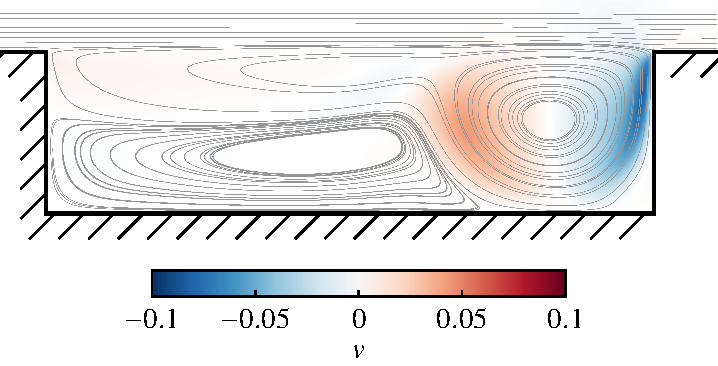
\includegraphics[width=\textwidth]{../../Images/gapd4_w15.pdf}
		\\
		\small{(a) Gap with $w=15\dstar$ and $d=4\dstar$.}
	\end{minipage}

	\vspace{0.3cm}

	\begin{minipage}{\linewidth}
		\centering
		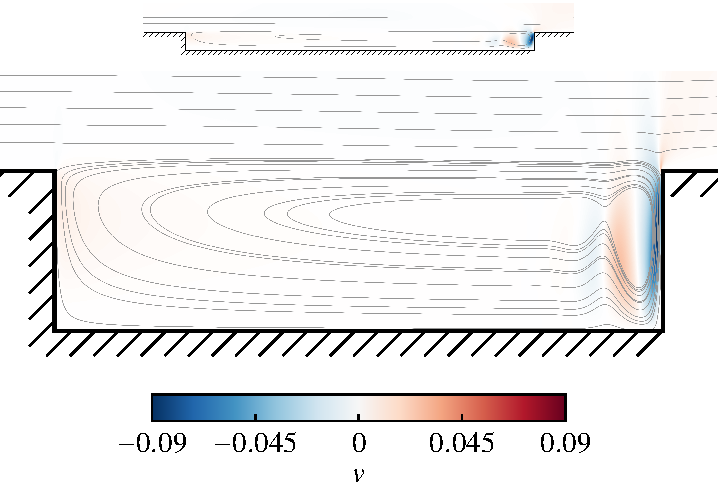
\includegraphics[width=\textwidth]{../../Images/gapd1.5_w30.pdf}
		\\
		\small{(b) Gap with $w=30\dstar$ and $d=1.5\dstar$.}
	\end{minipage}

	\vspace{0.3cm}

	\begin{minipage}{\linewidth}
		\centering
		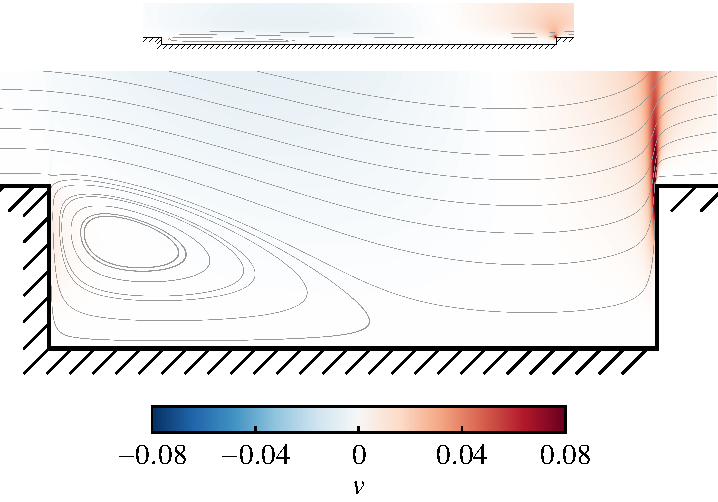
\includegraphics[width=\textwidth]{../../Images/gapd1_w60.pdf}
		\\
		\small{(c) Gap with $w=60\dstar$ and $d=1\dstar$.}
	\end{minipage}

	\caption{Equilibrium solutions for three representative geometries. Wall-normal-velocity contours and streamlines are shown. All geometries are rescaled to match the first case ($w/d = 15/4$) for visual comparison; original unscaled geometries are shown above the last two panels.}
	\label{fig:stableSS}
\end{figure}

For deep gaps, a pronounced recirculation region forms near the downstream cavity edge. For shallow gaps, this structure is absent; the flow enters and exits the cavity more smoothly, with only a weak upstream recirculation zone, resembling the flow over a backward-facing step.

At fixed depth, increasing width produces a sequence of bifurcations. Once $w$ exceeds a depth-dependent critical value $w_\text{c}$, the flow destabilizes. The first boundary in Figure~\ref{fig:2dstability} has been verified as a Hopf bifurcation for $d=3\dstar$, and the same bifurcation type is expected across the depths considered. The resulting stable limit cycle appears as a periodic oscillation localized near the downstream edge, acting as a blowing/suction-type source for the outer boundary layer. Its frequency $\omega_\text{2D}$ depends on depth: deep cavities exhibit relatively high frequency ($\omega_\text{2D}\simeq 0.24$) with rapid downstream decay, whereas shallow cavities ($d/\dstar\simeq 1.5$--$1.75$) exhibit lower frequency ($\omega_\text{2D}\simeq 0.10$), closer to TS-wave frequencies, and therefore generate longer convective structures. A representative state on this branch is shown in Figure~\ref{fig:absoluteInstability}.

For larger widths, attractors without a clear periodic signature emerge and are classified as chaotic. In the transition from limit-cycle to chaotic behavior, several intermediate scenarios are observed, including modal interaction across distinct frequencies, transient chaotic episodes that relaminarise to a different limit cycle, and period-doubling. The detailed route to chaos remains under investigation.

\begin{figure}[ht]
	\centering
	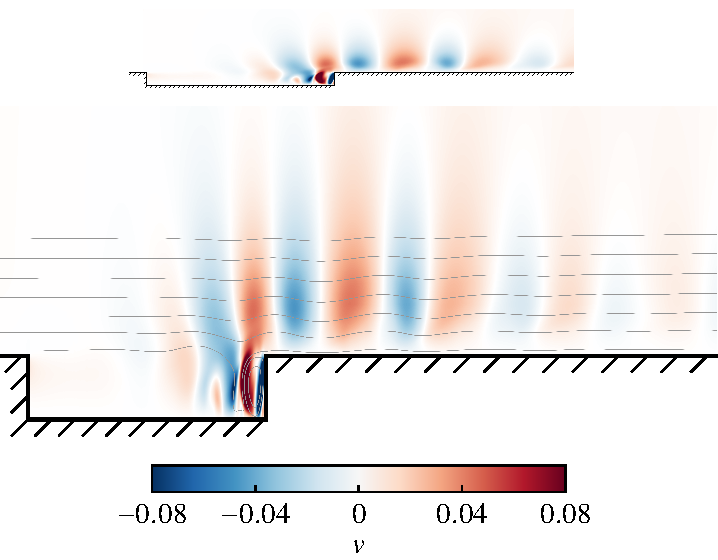
\includegraphics[width=\linewidth]{../../Images/gapd2.25_w35.pdf}
	\caption{Stable limit cycle for $w=35\dstar$ and $d=2.25\dstar$, visualized using wall-normal-velocity contours. The geometry is rescaled to $w/d=15/4$, with the original shape shown above for reference.}\label{fig:absoluteInstability}
\end{figure}

\section*{TS-WAVE AMPLIFICATION}
To corroborate the TS-wave amplification trends reported by~\cite{jeffGaps}, we perform linearised simulations around equilibrium base states $\mathbf{U}$ extracted from DNS. Because each base flow already satisfies the inhomogeneous boundary conditions, homogeneous conditions of the same type are imposed for the perturbation problem. TS waves are forced through a localized divergence-free body force in the upstream boundary layer, applied to both streamwise and wall-normal momentum components. The forcing is driven by white Gaussian noise, and the body force is
\begin{align}
	f_u(\mathbf{x},t) & = -(y-y_{\text{c}}) \expp{-\alpha[{(x-x_{\text{c}})}^2 + {(y-y_{\text{c}})}^2]} X_t, \\
	f_v(\mathbf{x},t) & = (x-x_{\text{c}}) \expp{-\alpha[{(x-x_{\text{c}})}^2 + {(y-y_{\text{c}})}^2]} X_t,
\end{align}
where $\alpha = 100$, $x_{\text{c}} = -95\dstar$, $y_{\text{c}} = 0.5\dstar$, and $X_t$ is unit-variance white Gaussian noise. The Gaussian envelope localizes excitation to an approximately circular region of radius $0.5\delta^*$ centered at $(x_{\text{c}},y_{\text{c}})$. Although experimental disturbances are neither white nor Gaussian, this idealized forcing is commonly used as a broadband and reproducible excitation model. The corresponding stability-analysis setup is shown in Figure~\ref{fig:pertdomain}.

\begin{figure}[ht]
	\centering
	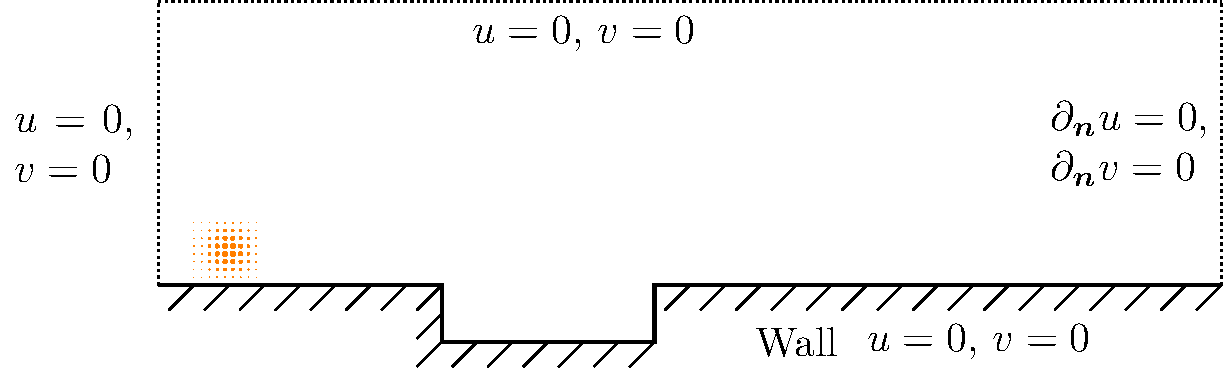
\includegraphics[width=\linewidth]{../../Images/domainPert.pdf}
	\caption{Domain used for stability analysis. White Gaussian forcing is applied in a localized upstream region (orange) to excite TS waves.}\label{fig:pertdomain}
\end{figure}
After forcing is introduced, the system is advanced through an initial transient until a statistically stationary response is reached. Temporal averaging is then performed to reduce stochastic variability in the measured wave amplitudes. TS-wave amplification is quantified using the $e^n$ method, which assumes that a disturbance with amplitude $A(x_0)$ at a reference location $x_0$ evolves as
\begin{equation}
	A(x) = A(x_0) \exp{n_{x_0}(x)},
	\label{eq:amplitudeEvolution}
\end{equation}
where $n_{x_0}(x)$ is the $n$-factor, obtained from
\begin{equation}
	n_{x_0}(x) = \log\left( \frac{A(x)}{A(x_0)} \right).
	\label{eq:nfactorAmplitude}
\end{equation}
Hereafter, the subscript $x_0$ is omitted for clarity. The disturbance amplitude is defined as the wall-normal $L^2$ norm of the perturbation velocity:
\begin{equation}
	A(x) := \norm{|\mathbf{u}'|}_{L^2(\mathcal{Y}(x))} = {\left( \int_{\mathcal{Y}(x)} u'^2 + v'^2 \dd{y}\right)}^{1/2},
	\label{eq:amplitudeNorm}
\end{equation}
where $\mathcal{Y}(x)$ denotes the wall-normal section at streamwise location $x$ and $\mathbf{u}' =(u',v')$ is the perturbation velocity field. Because the forcing is stochastic, the working amplitude in practice is the time-averaged RMS quantity
\begin{equation}
	A(x) := {\left( \int_{\mathcal{Y}(x)} \left\langle u_i'^2 + v_i'^2\right\rangle \dd{y}\right)}^{1/2}.
	\label{eq:amplitudeRMS}
\end{equation}
where $(u_i', v_i')$ are perturbation components at different time instances and $\langle \cdot \rangle$ denotes temporal averaging. The minimum perturbation amplitude upstream of the gap is used as reference to compute the $n$-factor curve through Equation~\ref{eq:nfactorAmplitude}. For simplicity, this curve is denoted by $n(x)$.

For comparison with~\cite{jeffGaps}, we evaluate the difference between the $n$-factor of each gapped case and that of the flat-plate reference. Because this difference exhibits mild streamwise variation, and because the objective is to isolate gap-induced TS-wave amplification rather than downstream evolution, we average over a $200\dstar$-long interval starting shortly downstream of the gap, at the onset of the slowly varying monotonic region of the $n$-factor curves, where the direct influence of the gap on amplification has effectively decayed. This metric is denoted $\Delta n$ (rather than $\Delta N$, as per~\cite{jeffGaps}) to emphasize that specific growth histories are compared rather than envelope maxima. Figure~\ref{fig:nfactorcountour}

The $\Delta n$ values are computed for all configurations that admit a stable equilibrium (i.e.\ laminar base flow). Interpolation within the convex hull is performed using a Gaussian-process regressor with a Mátern kernel. In Figure~\ref{fig:nfactorcountour}, dark blue solid lines denote the corresponding numerical predictions, and orange dashed lines denote experimental level curves from~\cite{jeffGaps} ($\Delta n=1,2,3,4,5$).

\begin{figure}[ht]
	\centering
	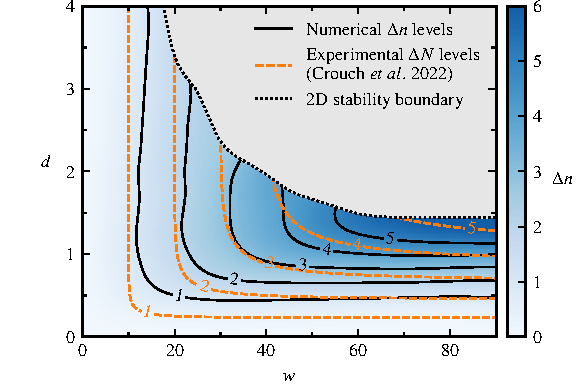
\includegraphics[width=\linewidth]{../../../images/DeltaNcountour.pdf}
	\caption{Contour map of $\Delta n$ on the stable side of the parameter grid $(w/\dstar,d/\dstar)\in[0,90]\times[0,4]$. Dark blue solid contours indicate the corresponding numerical predictions. Orange dashed contours indicate experimental levels from~\cite{jeffGaps} for $\Delta n=1,2,3,4, 5$. }\label{fig:nfactorcountour}
\end{figure}


Overall, the agreement with experiment is strong. In particular, both asymptotic trends are recovered: a predominantly vertical trend for narrow gaps and a predominantly horizontal trend for shallow gaps.

\section*{3D EFFECTS AND TRANSITION MECHANISMS}
Although the two-dimensional analysis captures the primary bifurcation structure, transition is inherently three-dimensional. We therefore extend the stability analysis to three dimensions by extruding the two-dimensional domain in the spanwise direction over a length $L_z$. Periodic boundary conditions are imposed in the span, and the solution is expanded in Fourier modes. The choice of $L_z$ (and thus spectral resolution in $z$) is discussed below.

To identify candidate three-dimensional instabilities, we first perform a single-mode linear stability analysis over a discrete set of spanwise wavenumbers, \(k_z = 2\pi/L_z\), with \(L_z/d \in [0.5,4]\). This provides an estimate of the most unstable spanwise wavenumber for each geometry. The resulting stability map is shown in Figure~\ref{fig:3dstability}.

\begin{figure}[ht]
	\centering
	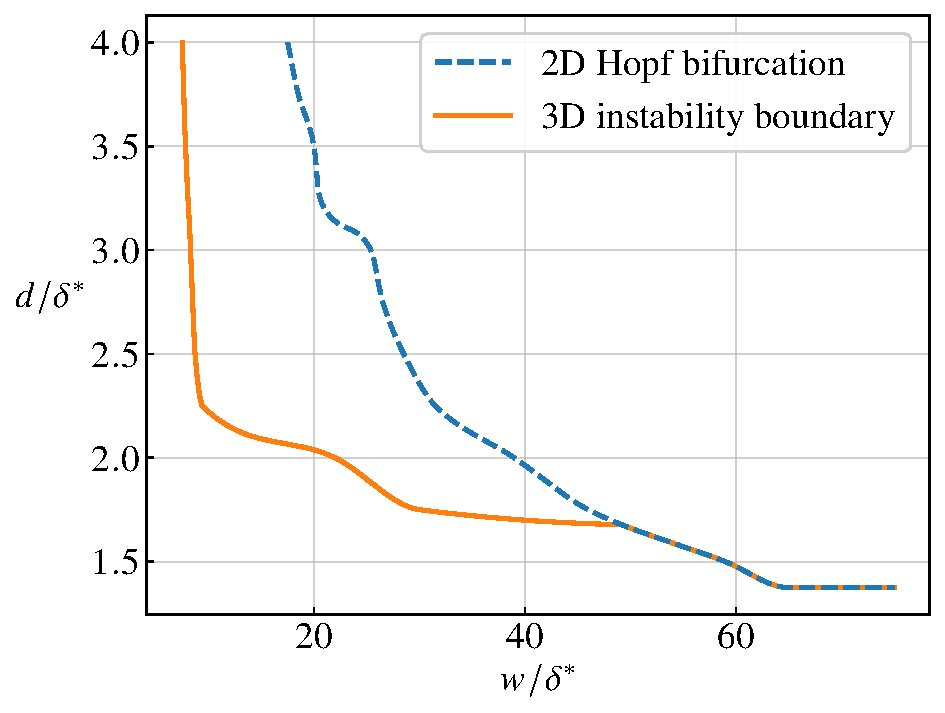
\includegraphics[width=\linewidth]{../../../images/3d2dbifurcations.pdf}
	\caption{Bifurcation boundaries for the 2D instability (Hopf bifurcation) and 3D instability.}\label{fig:3dstability}
\end{figure}

For deep gaps, the three-dimensional instability appears at smaller widths than the two-dimensional instability. For very shallow gaps, by contrast, the dominant dynamics remain effectively two-dimensional. To assess the implications for fully nonlinear transition, we ran three-dimensional simulations across representative cases using $L_z=4d$ and 32 complex Fourier modes. This spanwise extent is sufficient for the relevant instability range: the most unstable wavenumber is consistently close to $k_z=2\pi/(1.25d)$, while modes with $k_z \lesssim 2\pi/(3d)$ are damped. Figure~\ref{fig:3dmode} shows the most unstable mode for $w=14\dstar$, $d=4\dstar$, and $L_z=1.25d$. Relative to the two-dimensional limit cycle, this mode exhibits long but weak downstream streaks compared with the much stronger cavity-core response. Its frequency, $\omega_\text{3D}\simeq 0.025$, is about one order of magnitude lower than the two-dimensional frequencies $\omega_\text{2D}\simeq 0.10$--$0.24$.

\begin{figure}[ht]
	\centering
	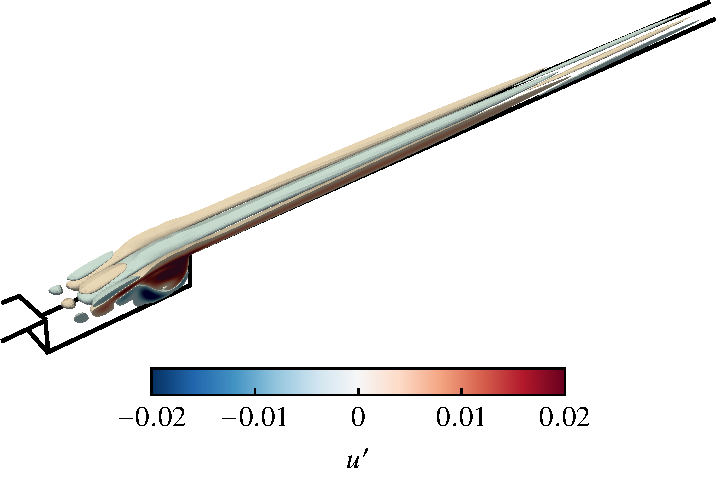
\includegraphics[width=\linewidth]{../../Images/3dModeParaview/main.pdf}
	\caption{Most unstable three-dimensional mode for $w=14\dstar$, $d=4\dstar$, and $L_z = 1.25d$.}\label{fig:3dmode}
\end{figure}

The full three-dimensional study considers $(w/\dstar, d/\dstar) \in \{(14,4), (19,4), (24,2), (40,2), (80,1.5)\}$. For $d=4\dstar$ and $d=2\dstar$, two widths are simulated: one below and one above the two-dimensional critical width $w_\text{c}$. For $d=1.5\dstar$, only a case with $w>w_\text{c}$ is considered because no separate three-dimensional bifurcation is detected.

Two distinct transition mechanisms are identified. For deep gaps ($d\geq 2\dstar$) with $w< w_\text{c}$, the three-dimensional instability perturbs the cavity dynamics but does not trigger rapid breakdown in the boundary layer: no persistent coherent pattern forms in the cavity, and downstream streaks remain too weak to induce near-field boundary-layer transition. For $w>w_\text{c}$, a two-dimensional oscillatory mode destabilizes first; the downstream boundary layer quickly organizes around this mode, after which secondary three-dimensionality grows and breakdown occurs close to the downstream edge. A representative deep-gap transition sequence is shown in Figure~\ref{fig:gapTransition}. For shallow gaps ($d\simeq 1.5\dstar$), no distinct three-dimensional instability is observed. Instead, the dominant response resembles a TS-wave mode, consistent with strong TS overamplification in this region of parameter space (Figure~\ref{fig:nfactorcountour}), leading to a classical downstream TS-wave transition scenario.
\begin{figure}[ht]
	\centering
	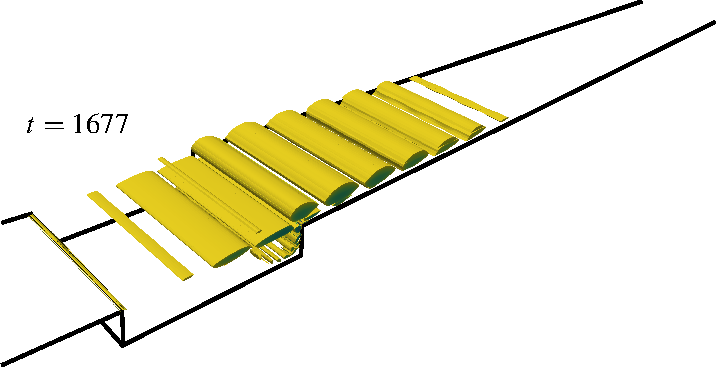
\includegraphics[width=\linewidth]{../../Images/3dTransParaview/pdfs/d4w19_3d_L2crit_10.pdf}\\[-0.5cm]
	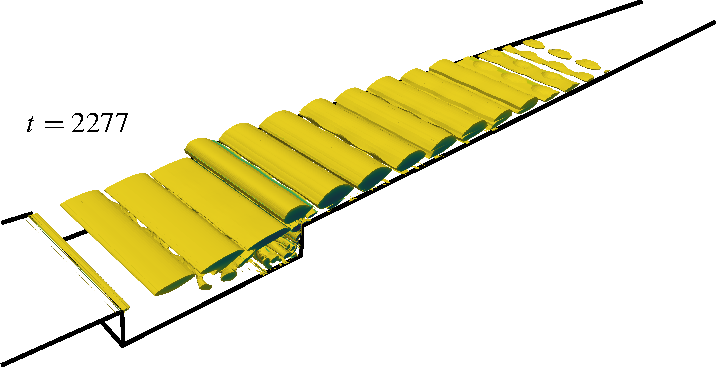
\includegraphics[width=\linewidth]{../../Images/3dTransParaview/pdfs/d4w19_3d_L2crit_12.pdf}\\[-1.5cm]
	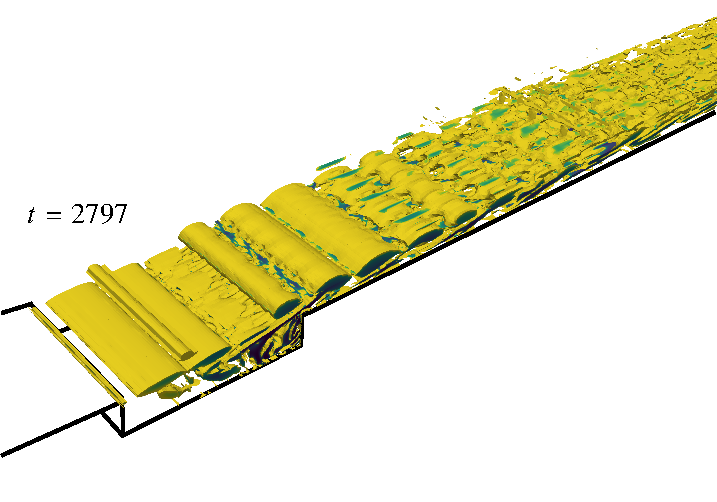
\includegraphics[width=\linewidth]{../../Images/3dTransParaview/pdfs/d4w19_3d_L2crit_14_big.pdf}\\[-2.65cm]
	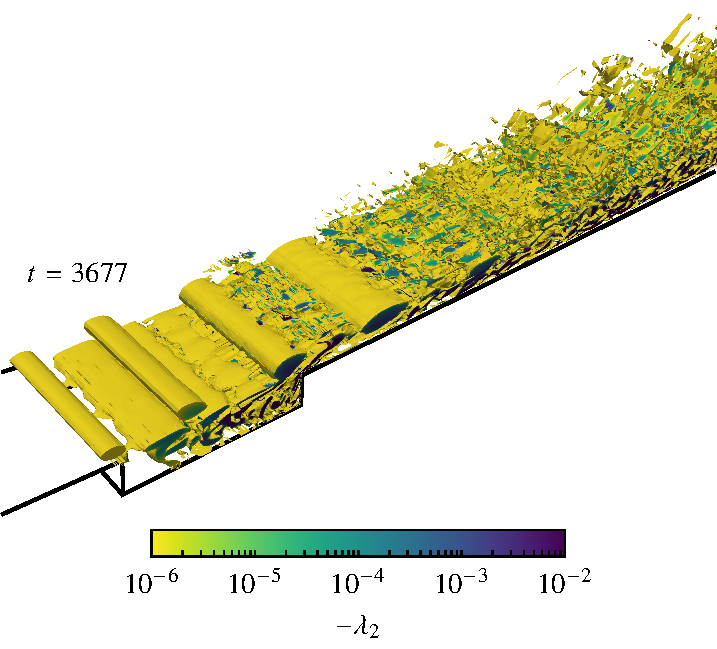
\includegraphics[width=\linewidth]{../../Images/3dTransParaview/pdfs/d4w19_3d_L2crit_17_big.pdf}
	\caption{Transition sequence for $w=19\dstar$ and $d=4\dstar$. Vortical structures are visualized using $\lambda_2$-criterion isosurface. The simulation time corresponding to each state is indicated next to each visualization.}\label{fig:gapTransition}
\end{figure}

\section*{MACH NUMBER INFLUENCE}
A set of compressible simulations is conducted to quantify the influence of Mach number on the two-dimensional Hopf bifurcation boundary.

Relative to the incompressible configuration, the principal change is the governing model: the compressible Navier--Stokes equations for an ideal gas. In nondimensional conservative form, these equations are
\begin{equation}
	\begin{aligned}
		\partial_t \rho + \grad \cdot (\rho \mathbf{u})                                              & = 0,                           \\
		\partial_t (\rho \mathbf{u}) +\grad \cdot (\rho \mathbf{u} \otimes \mathbf{u} + p\mathbf{I}) & = \grad \cdot \bm{\tau},       \\
		\partial_t E+\grad \cdot ((E+p)\mathbf{u})                                                   & =
		\grad \cdot \left(\boldsymbol{\tau} \cdot \mathbf{u} + \frac{\mu}{\Ma^2 \Pr (\gamma - 1)} \grad T\right),                     \\
		p                                                                                            & = \frac{\rho T}{\gamma \Ma^2},
	\end{aligned}
	% \begin{aligned}
	% 	\partial_t \rho &= \grad \cdot (\rho \mathbf{u})  0, \\
	% 	\partial_t (\rho \mathbf{u}) &= -\grad \cdot (\rho \mathbf{u} \otimes \mathbf{u} + p\mathbf{I})  + \grad \cdot \boldsymbol{\tau}, \\
	% 	\partial_t E &= -\grad \cdot ((E+p)\mathbf{u}) +
	% 	\grad \cdot \left(\boldsymbol{\tau} \cdot \mathbf{u} + \frac{\mu}{M^2 \Pr (\gamma - 1)} \grad T\right),
	% \end{aligned}
\end{equation}
where $\rho$ is density, $\mathbf{u} = (u,v)$ or $(u,v,w)$ is velocity, $p$ is pressure, $\otimes$ denotes the outer product, $\mathbf{I}$ is the identity tensor, and
\begin{equation}
	\bm{\tau} = \mu(\Rey) \left( \grad \mathbf{u} + \transpose{(\grad \mathbf{u})} - \frac{2}{3} (\grad \cdot \mathbf{u}) \mathbf{I} \right)
\end{equation}
is the viscous stress tensor under Stokes' hypothesis. Dynamic viscosity $\mu$ is evaluated using Sutherland's law:
\begin{equation}
	\mu =\frac{T^{3/2}}{\Rey} \frac{1 + S/T_\infty}{T + S/T_\infty},
\end{equation}
where $T$ is temperature, $S=110$\,K is Sutherland's constant, and $T_\infty$ is the reference temperature. Total energy is
\begin{equation}
	E = \frac{p}{\gamma - 1} + \frac{1}{2} \rho |\mathbf{u}|^2.
\end{equation}
The nondimensional control parameters are defined from free-stream reference quantities as
\[
	\Rey=\frac{\rho_\infty u_\infty \dstar}{\mu_\infty},\qquad
	\Ma=\frac{u_\infty}{\sqrt{\gamma R T_\infty}},\qquad
	\Pr=\frac{\mu_\infty c_p}{k_\infty},
\]
where the subscript $\infty$ denotes free-stream values. Here, $R$, $c_p$, and $k$ denote the specific gas constant, the specific heat at constant pressure, and the thermal conductivity, respectively. In the compressible simulations, $\Rey=1000$ (matching the incompressible study), $\Pr=0.72$, and $\gamma=1.4$ are held fixed, while $\Ma$ is varied over $\{0.05, 0.2, 0.4, 0.6, 0.8\}$.

A discontinuous Galerkin (DG) formulation is used, with weak DG advection, Roe upwinding for inter-element fluxes, and interior penalty treatment of diffusion. Polynomial order $p=3$ is used in each element, and time advancement uses a second-order diagonally implicit Runge--Kutta (DIRK) scheme (see~\cite{KENNEDY}).

The same geometric parameter space as in the incompressible analysis is considered: $w/\dstar \in [0,130]$ and $d/\dstar \in [0.25,4]$.

The instability structure remains qualitatively similar to the incompressible case: a depth-dependent critical width marks a Hopf onset. The resulting boundaries for different Mach numbers are shown in Figure~\ref{fig:MachBifurcation}.

\begin{figure}[ht]
	\centering
	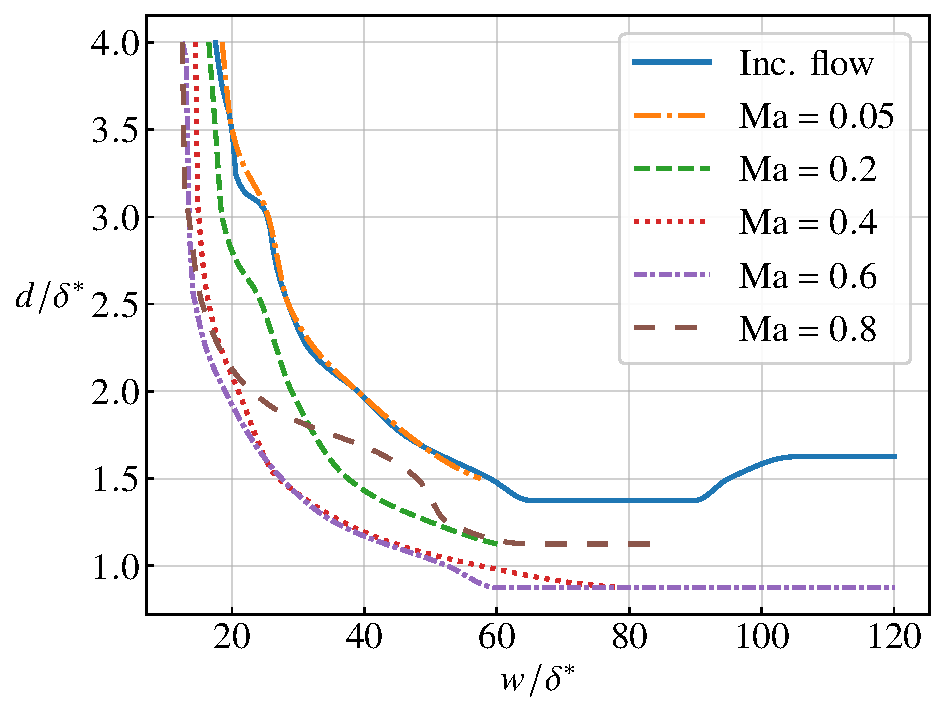
\includegraphics[width=\linewidth]{../../../images/Mabifurcations.pdf}
	\caption{Linear stability boundaries for the two-dimensional configuration at different Mach numbers.}\label{fig:MachBifurcation}
\end{figure}

Agreement between the $\Ma=0.05$ and incompressible boundaries is strong, supporting consistency between the incompressible and compressible solvers. As $\Ma$ increases, the bifurcation boundary generally shifts toward smaller widths, indicating a destabilizing compressibility effect, particularly for deep gaps. For shallow gaps ($d/\dstar \lesssim 2$), however, this trend is non-monotonic: at $\Ma=0.8$, the flow appears more stable than at intermediate Mach numbers ($\Ma=0.4$--$0.6$). The underlying mechanism for this partial restabilisation is not yet clear, and is the subject of ongoing investigation.

\section*{CONCLUSIONS}
This study presents a unified investigation of transition in laminar boundary layers over surface gaps using high-fidelity incompressible and compressible simulations, supported by linear stability analysis.

A systematic two-dimensional parameter study reveals a rich bifurcation structure. At fixed depth, increasing width beyond a critical threshold $w_\text{c}$ triggers a Hopf bifurcation and a stable limit cycle localized near the downstream edge. Further width increase leads to more complex dynamics, including period-doubling and chaotic attractors.

TS-wave amplification, quantified through $\Delta n$ within the $e^n$ framework, agrees closely with the measurements of~\cite{jeffGaps}. Both asymptotic regimes are recovered: depth-dominated behavior for shallow gaps and width-dominated behavior for narrow deep gaps.

Three-dimensional analysis shows that deep gaps admit a distinct low-frequency spanwise instability that can precede two-dimensional Hopf onset. Fully three-dimensional simulations indicate two transition routes: for deep gaps with $w>w_\text{c}$, rapid breakdown follows growth of the two-dimensional oscillatory mode and subsequent secondary three-dimensional instability; for shallow gaps, transition is governed by downstream TS-wave overamplification.

Compressible simulations show a clear Mach-number influence: increasing $\Ma$ generally shifts the bifurcation boundary toward smaller widths, i.e., destabilization. For shallow gaps, however, the highest Mach number considered ($\Ma=0.8$) produces partial restabilisation relative to intermediate $\Ma$, indicating a non-trivial compressibility--geometry interaction.

Overall, the results provide a coherent physical picture of gap-induced transition across two- and three-dimensional settings and clarify how compressibility modifies instability thresholds relevant to practical aerodynamic surfaces with manufacturing discontinuities.

\bibliographystyle{tsfp}
\bibliography{tsfp}

\end{document}
